\documentclass[a4paper,10pt]{article}
\usepackage[margin=0.53in]{geometry}
\usepackage{graphicx}
\usepackage{array}
\usepackage{enumitem}
\usepackage{titlesec}
\usepackage{setspace}
\usepackage{multicol}
\usepackage{ragged2e}
\usepackage[none]{hyphenat}
\usepackage{qrcode}

\renewcommand{\baselinestretch}{1.1}
\setlength{\parindent}{0pt}
\pagestyle{empty}

\begin{document}
\centering
\begin{tabular}{|l@{\hspace{1em}}|>{\raggedright\arraybackslash}p{12cm}|}

\hline
\multicolumn{2}{|p{18cm}|}{
\centering \textbf{PlantIQ: A Multimodal, Retrieval-Grounded Decision-Support Platform for Smallholder Coffee Growers in Karnataka}
\vspace{0.15cm}
} \\
\hline
\multicolumn{2}{|p{16cm}|}{
\textbf{Domain:} Deep Learning, Computer Vision, Retrieval-Augmented Generation, NLP, Agricultural Decision Support
\vspace{0.1cm}
} \\
\hline
\multicolumn{2}{|p{18cm}|}{
\textbf{Abstract:}\newline
\justifying
Coffee growers in the Chikkamagaluru, Kodagu and Hassan districts of Karnataka face three recurring problems: foliar diseases that spread quickly during the monsoon, treatment advice that is generic, English-only and blind to the day's weather, and weak access to buyers for small lots. PlantIQ is an Android and web platform backed by a self-hostable server, built as four modules. Module 1 diagnoses a single leaf photograph as leaf rust, Cercospora leaf spot, Phoma leaf spot, leaf miner or healthy with a transfer-learned ResNet-50 convolutional neural network, and a 75\% confidence gate flags uncertain photographs instead of guessing. Module 2 produces a treatment plan by retrieval-augmented generation over Central Coffee Research Institute (CCRI) extension documents and research papers: a hybrid retriever fuses multilingual dense search with BM25 keyword search, reranks with a cross-encoder and removes redundant passages; the large language model's advice is conditioned on live estate weather, a fungal infection-risk level and a three-day spray window, and every dose it states is checked against the retrieved passages. Module 3 is an English and Kannada chat assistant with conversation memory, photo hand-off and on-device speech recognition for Kannada and Indian English. Module 4 is a marketplace that normalises quantities and prices to kilograms and rupees per kilogram and ranks lots by distance. On the development laptop, leaf inference takes 5.3 ms on the GPU, retrieval about 0.4 s and a complete advisory about 6 s, and the system is covered by 354 automated tests. An audit of the public JMuBEN coffee-leaf dataset found that its 58,549 images come from only 861 distinct leaf patches, so a random split leaks almost every test image into training; models are therefore compared with leak-free, group-aware cross-validation against re-implemented baselines from prior coffee-disease work.
} \\
\hline
\multicolumn{2}{|p{16cm}|}{
\begin{minipage}[t]{\linewidth}
\textbf{Architecture / Flow Diagram:}

\vspace{6pt}
\end{minipage}
} \\
\multicolumn{2}{|c|}{
  \begin{minipage}{\linewidth}
    \centering
    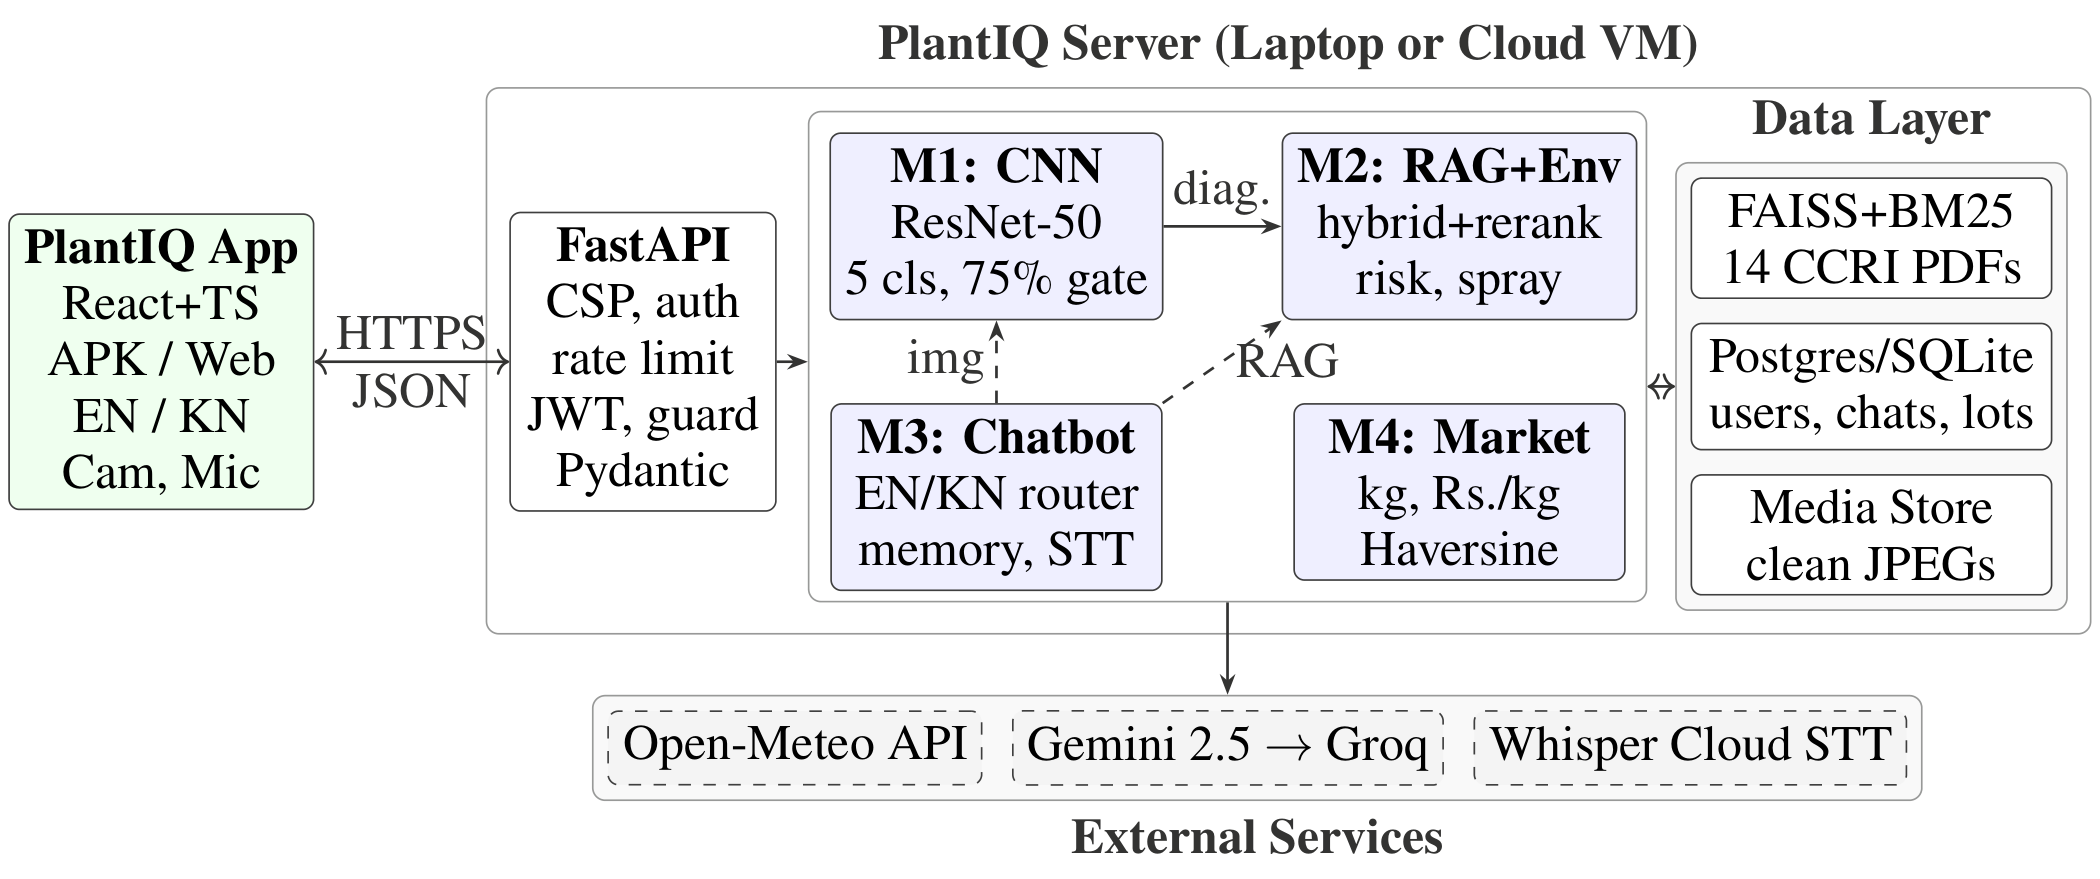
\includegraphics[width=13.5cm]{35_1.png}\\[6pt]
    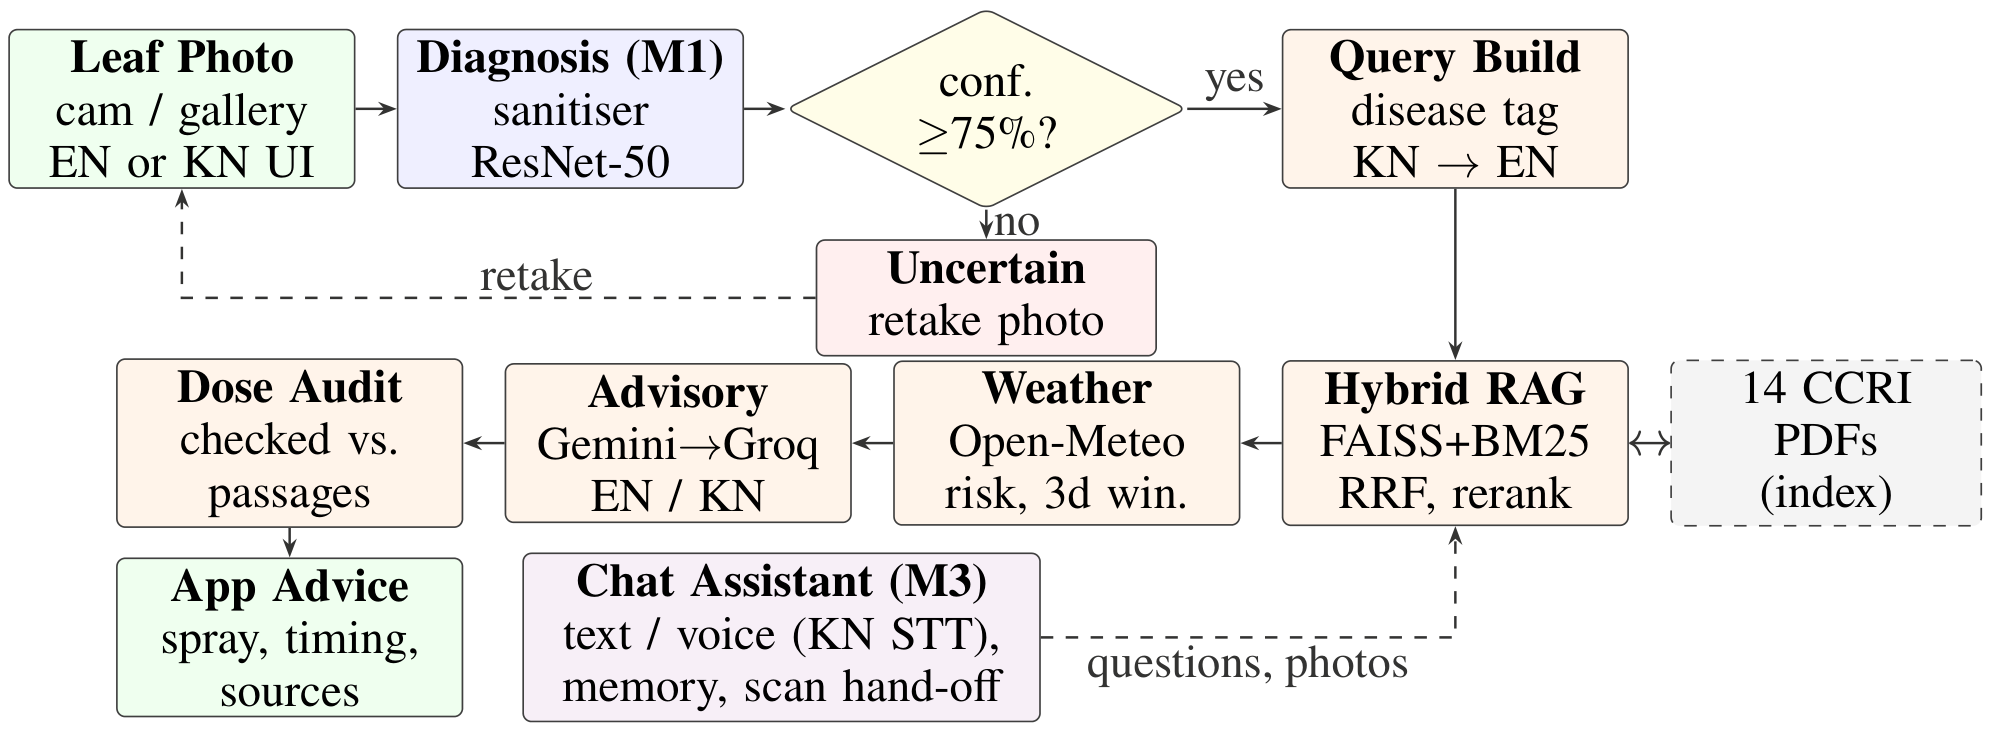
\includegraphics[width=13.5cm]{35_2.png}
    \vspace{6pt}
  \end{minipage}
} \\

\hline
\begin{tabular}[t]{@{}l@{}}
\textbf{Supervisor:} \\[0.8ex]
Prof. Deepti C. \\[-0.1em]
\small Assistant Professor, Dept. of CSE
\end{tabular}
&
\begin{tabular}[t]{@{}l@{}}
\textbf{Team No.:} 35 \\[0.8ex]
\begin{tabular}[t]{@{}l l l@{}}
\small\textbf{Jeel Nada} & \small\textbf{Nidhi N Udupa} & \small\textbf{Mohammed Ayaan} \\
\small PES2UG23CS357 & \small PES2UG23CS384 & \small PES2UG23AM058 \\
\end{tabular}
\end{tabular} \\
\hline

\multicolumn{2}{|p{16cm}|}{
\textbf{Publication:}
} \\
\multicolumn{2}{|p{18cm}|}{
  \begin{tabular}{@{}p{13.5cm} p{3.5cm}@{}}
    \textbf{Status:} Under preparation (target: IEEE conference)\newline
    
    \raggedright Jeel Nada, Nidhi N Udupa, Mohammed Ayaan and Prof.~Deepti C. (2026). PlantIQ: A Multimodal, Retrieval-Grounded Decision-Support Platform for Smallholder Coffee Growers in Karnataka. Manuscript in preparation. Project source code: github.com/jeelnadaa/plantiq-capstone
    &
    \makebox[3.5cm][c]{\raisebox{-0.8\height}{\qrcode[height=2.2cm]
    % QR links to the project repository (the paper is not yet published)
    {https://github.com/jeelnadaa/plantiq-capstone}}}
  \end{tabular}

} \\

\hline
\end{tabular}

\end{document}
